\hsection{Problem Instance Data}%
\label{sec:problemInstance}%
%
\hsection{Definitions}%
%
We distinguish optimization \emph{problems} (see \autoref{def:optimizationProblemMathematical}) from \emph{problem instances}.
An optimization problem is the general blueprint of the tasks.
The \gls{JSSP}, for instance, has the goal of scheduling production jobs to machines under a set of constraints that we will discuss later.
A problem instance of the \gls{JSSP} is a concrete scenario, e.g., a concrete lists of tasks, requirements, and machines.%
%
\begin{definition}%
\label{def:instance}%
A concrete instantiation of all information that are relevant from the perspective of solving an optimization problems is called a \emph{problem instance}~\instance.%
\end{definition}%
%
The problem instance is the \emph{input} of the optimization algorithms.
A problem instance is related to an optimization problem in the same way an object/instance is related to its \codeil{class} in an object-oriented programming language like Python or Java, or a \codeil{struct} in~C.
The \codeil{class} defines which member variables exist and what their valid ranges are.
An instance of the \codeil{class} is a piece of memory which holds concrete values for each member variable.%
%
\endhsection%
%
\hsection{Example: Job Shop Scheduling}%
\label{sec:jsspInstance}%
%
\hsection{JSSP Instance Structure}%
\label{sec:jsspInstanceStructure}%
%
So how can we characterize a \gls{JSSP} instance~\instance?
In the basic and yet general scenario~\cite{GLLRK1979OAAIDSASAS,LLRKS1993SASAAC,L1982RRITTOMS,T1993BFBSP}, our factory has~$\jsspMachines\in\naturalNumbersZ$ machines.
At each point in time, a machine can either work on exactly one job or do nothing (be idle).
A job may correspond to a customer order, e.g., \inQuotes{produce 10 red lady's sneakers.}
There are~$\jsspJobs\in\naturalNumbersO$ jobs that we need to schedule to these machines.
For the sake of simplicity and for agreement between our notation here, the Python source code, and the example instances that we will use, we reference jobs and machines with 0\nobreakdash-based indices from~$\intRange{0}{(\jsspJobs-1)}$ and~$\intRange{0}{(\jsspMachines-1)}$, respectively.

Each of the~\jsspJobs\ jobs is composed of~\jsspMachines\ \inQuotes{operations} --- one for each machine.
These operations correspond to the single production steps, such as \inQuotes{cut the cloth material,} \inQuotes{stitch the cloth material to the sole,} and so on.
Each job may need to pass through the machines in a different order.
The operation~\jsspMachineIndex\ of job~\jsspJobIndex\ must be executed on machine~$\jsspOperationMachine{\jsspJobIndex}{\jsspMachineIndex}\in \intRange{0}{(\jsspMachines-1)}$.
Doing so needs~$\jsspOperationTime{\jsspJobIndex}{\jsspMachineIndex}\in\naturalNumbersZ$ time units for completion.
Once a machine~\jsspMachineIndex\ begins to process an operation, it cannot stop until the operation is completed, i.e., will remain busy for~$\jsspOperationTime{\jsspJobIndex}{\jsspMachineIndex}\in\naturalNumbersZ$ time units.

This definition of a \gls{JSSP} instance~\instance\ is quite versatile.
For example, assume that we have a factory that produces exactly one single product, but different customers may order different quantities of this product.
Then, we would have \gls{JSSP} instances where all jobs need to be processed by exactly the same machines in exactly the same sequence.
In this case~$\jsspOperationMachine{\jsspJobIndex_1}{\jsspMachineIndex}=\jsspOperationMachine{\jsspJobIndex_2}{\jsspMachineIndex}$ would hold for all jobs~$\jsspJobIndex_1$ and~$\jsspJobIndex_2$ and all operation indices~\jsspMachineIndex.
The jobs would pass through all machines in the same order but may have different processing times (due to the different quantities).

We may also have scenarios where customers can order different types of products, say the same liquid soap, but either in bottles, plastic bags, or big canisters.
Then, different machines may be needed for different orders.
This is similar to the situation illustrated in \autoref{fig:jssp_sketch}, where some job~\jsspJobIndex\ does not need to be executed on a machine~$\jsspMachineIndex'$ while another does.
We then can simply set the required time~$\jsspOperationTime{\jsspJobIndex}{\jsspMachineIndex}$ to~0 for the operation~$\jsspMachineIndex$ with~$\jsspOperationMachine{\jsspJobIndex}{\jsspMachineIndex}=\jsspMachineIndex'$.
Notice that for this reason we wrote \inQuotes{$\jsspOperationTime{\jsspJobIndex}{\jsspMachineIndex}\in\naturalNumbersZ$} above, because $\naturalNumbersZ$ includes~0.

In other words, the \gls{JSSP} instance structure described here already encompasses a wide variety of real-world production situations.
If we can build an algorithm which can solve this general type of \gls{JSSP} well, it can automatically also solve the above-mentioned special cases.
\endhsection%
%
\hsection{JSSP Benchmark Instances}%
\label{sec:jsspBenchmarkInstances}%
%
In order to practically play around with optimization algorithms for a certain problem, we need concrete instances of that problem.
If we want to know whether an algorithm for the \gls{TSP} works well, then we need some \gls{TSP} instances, e.g., maps with the cities that we want to visit.

If we want to explore how different algorithms for the \gls{JSSP} perform, then we need some concrete instances of the \gls{JSSP}.
Obviously, if we want to know whether an algorithm~$\mathcal{A}$ is better than an algorithm~$\mathcal{B}$, then we need to apply them to the same problem instance.
Results obtained for different scenarios are inherently incomparable.

Luckily, the optimization community provides \inQuotes{benchmark instances} for many different optimization problems.
Such common, well-known instances are important, because they allow researchers to compare their algorithms.

The eight classical and most commonly used sets of benchmark instances for the \gls{JSSP}~\cite{H2002PJSSP} are published in~\cite{FT1963PLCOLJSSR,ABZ1988TSBPFJSS,AC1991ACSOTJSSP,SWV1992NSSFSPWATJSS,YN1992AGAATLSJSI,L1998RCPSAEIOHSTS,DMU1998BFSSP,T1993BFBSP}.
Their data can be found (sometimes partially) in several repositories in the Internet, such as%
%
\begin{itemize}%
%
\item the OR\nobreakdash-Library managed by \citeauthorfull{B1990OLDTPBEM}~\cite{B1990OLDTPBEM},%
%
\item the comprehensive set of \gls{JSSP} instances provided by \citeauthorfull{vH2015JSIAS}~\cite{vH2015JSIAS,vH2018TCSOBOBIOTJSSP}, where also state-of-the-art results are listed,%
%
\item \citeauthorfull{S2019JSSPH}'s Page~\cite{S2019JSSPH}, which, too, contains up-to-date experimental results,%
%
\item \citeauthorfull{T1993SI}'s Page~\cite{T1993SI}, or, finally,%
%
\item my own repository \href{http://github.com/thomasWeise/jsspInstancesAndResults}{jsspInstancesAndResults}~\cite{W2019JRDAIOTJSSP}, where I collect all the above problem instances and many results from existing works.%
%
\end{itemize}%
%
We will try to solve \gls{JSSP} instances obtained from these collections.
The goal of this book is that you can play around with the algorithms and replicate our experiments.
Therefore, we cannot use all 242~instances from the above sets, because then the experiments would take too long.
We have to pick a small representative subset of instances.
We therefore first removed 67~instances that are relatively easy from the instance set.
We then picked instances with different scales and from different sources.
They will serve as illustrative example of how to approach optimization problems.
In order to keep the example and analysis simple, we will focus on only eight instances, namely%
%
\begin{enumerate}%
%
\item Instance \instStyle{abz8} by \citeauthor{ABZ1988TSBPFJSS}~\cite{ABZ1988TSBPFJSS} has 20~jobs and 15~machines.
The processing times of its operations were chosen from the interval~$\intRange{11}{40}$.%
%
\item Instance \instStyle{dmu67} by \citeauthor{DMU1998BFSSP}~\cite{DMU1998BFSSP} has 40~jobs and 20~machines.
Its processing times were chosen from the interval~$\intRange{1}{200}$.
This instance is structured such that the jobs first need to pass one (randomly chosen) half of the machines and then the other.%
%
\item Instance \instStyle{dmu72} is from the same group and has the same structure as \instStyle{dmu67}, but has 50~jobs and 15~machines.%
%
\item Instance \instStyle{la38} by \citeauthor{L1998RCPSAEIOHSTS}~\cite{L1998RCPSAEIOHSTS} has 15~jobs and 15~machines.
Its processing times are from~$\intRange{5}{99}$.%
%
\item Instance \instStyle{orb06} by \citeauthor{AC1991ACSOTJSSP}~\cite{AC1991ACSOTJSSP} has 10~jobs and 10~machines.
It was generated in 1986 as part of a set of \inQuotes{specially generated tougher problems}~\cite{JM1999DJSSPPAF,H2002PJSSP}.
Nevertheless, it will be the smallest instance in our experiments.%
%
\item Instance \instStyle{swv14} by \citeauthor{SWV1992NSSFSPWATJSS}~\cite{SWV1992NSSFSPWATJSS} has 50~jobs and 10~machines.
Its processing times are from the interval~$\intRange{1}{100}$.
Like in the case of \instStyle{dmu72}, the jobs first need to pass one (randomly chosen) half of the machines and then the other.%
%
\item Instance \instStyle{ta70} by \citeauthor{T1993BFBSP}~\cite{T1993BFBSP} has 50~jobs and 20~machines.
Its processing times are from the interval~$\intRange{1}{99}$.%
%
\item Instance \instStyle{yn4} by \citeauthor{YN1992AGAATLSJSI}~\cite{YN1992AGAATLSJSI} has 20~jobs and 20~machines.
Its processing times are from the interval~$\intRange{10}{50}$.%
%
\end{enumerate}%
%
The raw data of these instances is part of the \moptipy\ Python package with the sources for our experiments as resource.

Of course, if we really want to solve a new type of problem, we will normally use as many benchmark problem instances as possible to get a good understand about the performance of our algorithm(s).
Only for the sake of clarity of presentation, we will here limit ourselves to the above eight problems.
We have chosen them as hopefully diverse representatives of all of the common \gls{JSSP} benchmarks.
They stem from instance sets contributed by different researchers and have different numbers of jobs and machines.%
%
\endhsection%
%
\hsection{File Format and \instStyle{demo} Instance}%
\label{sec:jsspDemoInstance}%
Our benchmark instances for the \gls{JSSP} are taken from the OR\nobreakdash-Library.
In the simple text format used in the OR\nobreakdash-Library, several problem instances can be contained in one file.
For the sake of simplicity, we created one additional, smaller \gls{JSSP} instance to describe the format of these files, as illustrated in \autoref{fig:jssp_demo_instance}.

\begin{figure}%
\centering%
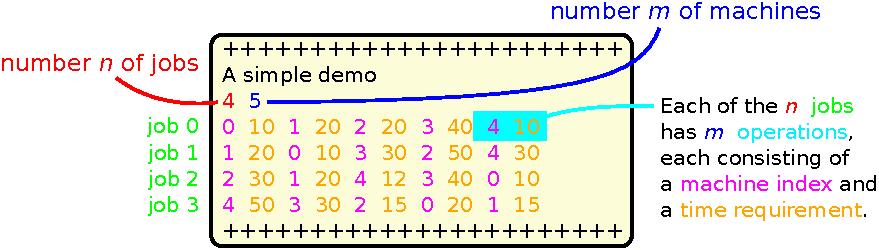
\includegraphics[width=0.9\linewidth]{\currentDir/jssp_demo_instance}%
\caption{The meaning of the text representing our \instStyle{demo} instance of the \gls{JSSP}, as an example of the format used by the OR-Library.}%
\label{fig:jssp_demo_instance}%
\end{figure}

Each problem instance~\instance\ starts and ends with a line of several \texttt{+} characters.
The next line is a short description or title of the instance.
In the third line, the number~\jsspJobs\ of jobs is specified, followed by the number~\jsspMachines\ of machines.
The actual IDs or indexes of machines and jobs are 0\nobreakdash-based, similar to array indices in Python.
The \gls{JSSP} instance definition is completed by~\jsspJobs\ lines of text.
Each such line specifies the operations of one job~$\jsspJobIndex\in\intRange{0}{(\jsspJobs-1)}$.
Each operation~\jsspMachineIndex\ is specified as a pair of two numbers, the ID~$\jsspOperationMachine{\jsspJobIndex}{\jsspMachineIndex}$ of the machine that is to be used ({\color{jssp-machine}violet}), from the interval~$\intRange{0}{(\jsspMachines-1)}$, followed by the number of time units~$\jsspOperationTime{\jsspJobIndex}{\jsspMachineIndex}$ the job will take on that machine ({\color{jssp-time}orange}).
The order in which these operations appear in a line defines exactly the order in which the job needs to be passed through the machines.
Of course, each machine can only process at most one job at a time.

In our demo instance illustrated in \autoref{fig:jssp_demo_instance}, this means that we have~$\jsspJobs=4$ jobs and~$\jsspMachines=5$ machines.
Job~0 first needs to be processed by {\color{jssp-machine}machine~0} for {\color{jssp-time}10~time units}, it then goes to {\color{jssp-machine}machine~1} for {\color{jssp-time}20~time units}, then to {\color{jssp-machine}machine~2} for {\color{jssp-time}20~time units}, then to {\color{jssp-machine}machine~3} for {\color{jssp-time}40~time units}, and finally to {\color{jssp-machine}machine~4} for {\color{jssp-time}10~time units}.
This job will thus take $10+20+20+40+10=100$~time units to be completed, \emph{if} it can be scheduled without any delay or waiting period, i.e., if all of its operations can directly be processed by their corresponding machines.
Job~3 first needs to be processed by machine~4 for 50~time units, then by machine~3 for 30~time units, then by machine~2 for 15~time units, then by machine~0 for~20 time units, and finally by machine~1 for 15~time units.
It would not be allowed to first send Job~3 to any machine different from machine~4 and after being processed by machine~4, it must be processed by machine~3 --- although it may be possible that it has to wait for some time, if machine~3 would already be busy processing another job.
In the ideal case, job~3 could be completed after 130~time units.
\endhsection%
%
\hsection{A Python Class for JSSP Instances}%
This structure of a \gls{JSSP} instance can be represented by the simple Python class.

What kind of information should the class provide?
Obviously, it needs to give us the machine data~\jsspOperationMachineMat\ and the time data~\jsspOperationTimeMat\ data.
To make working with these data easier, it should also tell us the number~\jsspMachines\ of machines and the number~\jsspJobs\ of jobs.
And since we are working with well-known benchmark instances, we should also store the names of the instances.

The first design choice that we will have to make is whether we represent \jsspOperationMachineMat\ and \jsspOperationTimeMat\ as separate matrices,  as one single \inQuotes{interleaved} matrix (like in the OR\nobreakdash-Library format illustrated in \autoref{fig:jssp_demo_instance}), or in a different way.
Either choice is OK, but here I chose the latter.

I chose to put the data into a three-dimensional array:
Each \codeil{Instance} is an array with one row for each job, one column for each operation, and each cell holds two values with the machine and the time spent on the machine.
In other words, an $\instance\relax[\jsspJobIndex, \jsspMachineIndex, 0]$ holds the machine~$\jsspOperationMachine{\jsspJobIndex}{\jsspMachineIndex}$ for the operation~$\jsspMachineIndex$ of job~$\jsspJobIndex$.
$\instance\relax[\jsspJobIndex, \jsspMachineIndex, 1]$ holds the time~$\jsspOperationTime{\jsspJobIndex}{\jsspMachineIndex}$ that job~$\jsspJobIndex$ will spend on machine~$k$.
This is still fairly close to the OR\nobreakdash-Library text format, while, at the same time, absolves me from fiddling around with the column index to figure out whether it points to a machine or a time.
By using the third dimension, I can immediately see this.

Of course, I could also have two separate matrices or use the same format as the text files.
This would mean that the code accessing the data would look a bit differently, but that would also be OK.

Now, if we want to represent matrices of integer values in Python, it is best to use \numpyndarrays.
These are memory efficient and accessing their elements is faster than using two-dimensional lists.
So we will make our class inherit from \numpyndarray.
We will also add an attribute \codeil{name} with the instance name stored as string.
Purely for the sake of simplicity, we also add the attributes \codeil{jobs} and \codeil{machines}, storing the number~\jsspJobs\ of jobs and the number~\jsspMachines, respectively.

\moptipyCode{moptipy/examples/jssp/instance.py}{--labels book --args doc,hints,comments}{jssp_instance}{Excerpt from a Python class for representing the data of a \gls{JSSP} instance.}

In \autoref{lst:jssp_instance}, we give an excerpt of this class, i.e., a snippet of the original code where some methods and data verification has been omitted.
We add a static method \codeil{from_resource(name)} to this class that can load any of the aforementioned benchmark \gls{JSSP} instances from a resource inside our \moptipy\ package directly based on its name (and return it as instance of \codeil{Instance}).
This way, we can conveniently access all the necessary data of a job shop scheduling task.
The actual code of the above, other utility methods, as well as sanity checks in the \codeil{__new__} constructor have here been omitted as they are unimportant for the understanding of the scenario.%
\endhsection%
\endhsection%
%

